\begin{quote}
Ten potentially useful things to do when you're solving a problem are
described by Artificial Intelligence pioneer Marvin Minsky in a series
of
\href{http://web.media.mit.edu/~minsky/OLPC-1.html}{m}\href{http://web.media.mit.edu/~minsky/OLPC-2.html}{e}\href{http://web.media.mit.edu/~minsky/OLPC-3.html}{m}\href{http://web.media.mit.edu/~minsky/OLPC-4.html}{o}\href{http://web.media.mit.edu/~minsky/OLPC-5.html}{s}
for the One Laptop Per Child project. We can sum them up visually with
the following diagram:
\end{quote}
\begin{center}
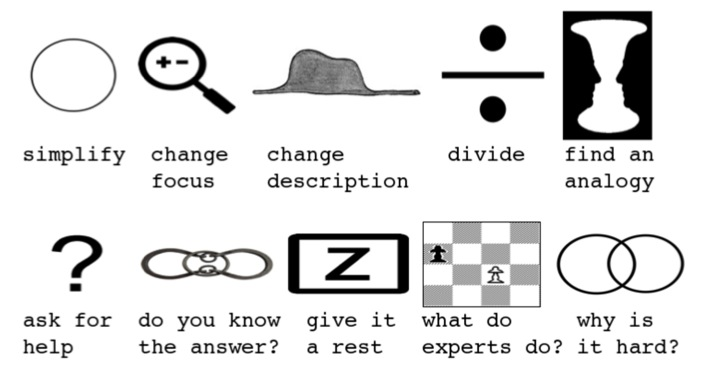
\includegraphics[width=\textwidth]{../pictures/heuristic-images.jpg}
\end{center}
We can also see some interesting relationships to the peeragogy patterns
we identified earlier. The connections are first described with a
picture here, and then in more detail with text below. Some of the nodes
in this diagram are clickable, and clicking will take you to the page
describing the relevant pattern:

To elaborate in words:

\begin{itemize}
\item
  Simplify things for \textbf{Newcomers}. In practice, this means that
  we don't expect a newcomer to enter at full speed.
\item
  Use a \textbf{Roadmap}to guide us from one phase to another, while the
  project's central \textbf{Heartbeat} helps us attend to the central
  focus.
\item
  Announce changes through a \textbf{Wrapper} who describes the new
  status or direction of the project. For the Peeragogy project, that
  often meant summing up the high points that we saw over a given period
  of time.
\item
  Assemble a \textbf{Pattern Language}for the project by first
  \textbf{Discerning Patterns}, and when we've seen how the patterns
  relate to each other (as in the diagram above), we can start to build
  a map like the one above, for subsequent use in problem-solving and
  design.
\item
  We divide work up not only horizontally among different
  \textbf{Roles}, but also temporally by using the \textbf{Roadmap}.
  Someone who is moving ahead with the Roadmap is likely to be working
  at the leading edge.
\item
  When we find an analogy, we are basically \textbf{Creating a Guide} of
  some sort. This can be used as a form of ``exploration,'' as we look
  at how one form of engagement may or may not map onto other forms of
  engagement.
\item
  When we ask for help, we may avail ourselves of some
  \textbf{Moderation} service that will decide how to deal with our
  request. One simple way to ask for help is \textbf{Polling for Ideas}.
  Obviously once we start to get help, we're working in a regime of
  ``collaborative effort''.
\item
  If you know the answer, then you may be able to reuse it (which is the
  basic idea described in \textbf{Praxis vs Poesis}, though the title is
  a little bit obscure). Someone who knows the answer and who is good at
  self-explanation may also have a good idea about how to get from the
  current state to the goal state; alternatively, this may be broken
  down into steps in some sub-Roadmap, and moving from step to step
  would then illustrate ``progressive problem solving''.
\item
  It is important to give it a rest so as not to over-exhaust oneself,
  busting one's own \textbf{Carrying Capacity}, or, alternatively,
  overwhelming the group.
\item
  It seems that one of the things that experts do is \textbf{Discerning
  a Pattern}. This allows them to simplify their processing.
\item
  Finally, again, if we know why it is hard, then we may be able to
  \textbf{Create a Guide} that will help get around, or at least better
  cope with, the difficulty.
\end{itemize}
\subsubsection{Resources}

\begin{itemize}
\item
  \emph{The Society of Mind} is a book by Marvin Minsky that talks about
  how a mind can be made up of many different ``agencies'' that work
  together. A relatively recent review by Push Singh is
  \href{http://web.media.mit.edu/~push/ExaminingSOM.html}{available
  online}, and contains a succinct overview of the key components of the
  more complex problem solving or ``thinking'' architecture described in
  Minsky's book.
\item
  \href{http://metameso.org/~joe/thesis-outline.html}{Peer Supported
  Problem Solving and Mathematical Knowledge} is a forthcoming Ph. D.
  thesis by peeragogy co-author Joseph Corneli.
\item
  Our \href{http://peeragogy.org/style-guide/}{Style Guide} contains
  some guidelines to use when working on ``problems of exposition''
\end{itemize}
